\namedchapter[Adam Zieliński]{Sterownik silników}
Sterownik silników został zaimplementowany na dwóch mikrokontrolerach z rodziny AVR. Każdy z nich sterowany jest przy wykorzystaniu osobnego układu. Realizacja regulatora wymaga obsługi pętli sprzężenia zwrotnego od prędkości obrotowej, zgodnie z schematem przedstawionym na rysunku \ref{schem_ster}. 

  \begin{figure}[H]
    \begin{center}
      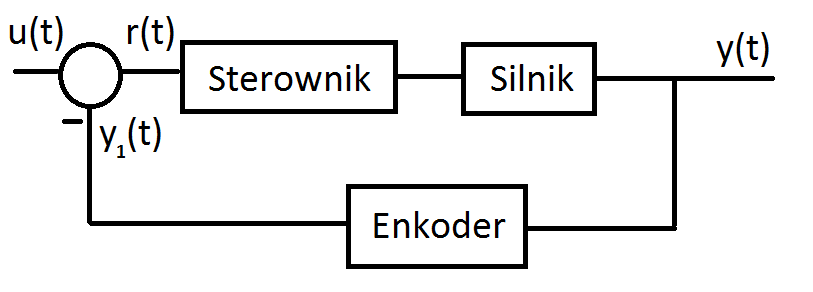
\includegraphics[scale=0.45]{imgs/sterowanie.png}
 	\caption[Schemat pętli sterowania silnikami.]{\small{Schemat przedstawia koncepcję pętli sterowania silnikami napędowymi. Ujemne sprzężenie zwrotne realizowane jest przy wykorzystaniu enkodera impulsowego. Sygnały: $u(t)$ - wartość zadana, $r(t)$ - uchyb, $y(t)$ wyjście układu, $y_1(t)$ - sygnał wyjściowy enkodera.}}
	\label{schem_ster}
    \end{center}
  \end{figure}  
  
\namedsection{Programowanie}
Programowanie Atmeg odbywa się przy wykorzystaniu programatora, czyli specjalnego układu elektronicznego służącego do sprzęgnięcia komputera z mikrokontrolerem zgodnie z rysunkiem \ref{schem_prog}. Urządzenie realizuje komunikację jednostronną, tzn. przesyła jedynie program do wewnętrznej pamięci układu scalonego.  Transmisja odbywa się przy wykorzystaniu magistrali SPI (ang. \textit{Serial Peripheral Interface}), która ,,wybiera" układ docelowy przy pomocy linii SS (ang. \textit{Slave Select}), następnie przesyła dane wykorzystując linie MISO (ang. \textit{Master Input Slave Output} - przyjmowanie danych), MOSI (ang. \textit{Master Output Slave Input} - nadawanie danych). Linia SCK służy do synchronizacji przebiegów szeregowych. Z racji tego, że programowany jest tylko jeden, aktualnie podłączony układ, linię SS można zaniechać.

  \begin{figure}[H]
    \begin{center}
      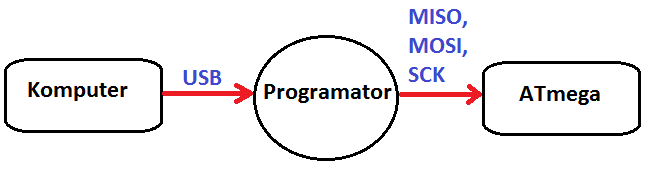
\includegraphics[scale=0.7]{imgs/schemat_prog.png}
 	\caption[Podłączenie programatora.]{\small{Graf przedstawiający idee pracy programatora. ATmega przyjmuje dane posługując się następującymi pinami : MISO, MOSI oraz SCK - zegar taktujący. Wymienione piny pozwalają na realizacje transmisji typu SPI pozwalającej na komunikacje jednostki centralnej z układami peryferyjnymi.}}
	\label{schem_prog}
    \end{center}
  \end{figure}  
  
\namedsection{Prędkość obrotowa}
Częstotliwość obrotu jest mierzona przy wykorzystaniu enkodera impulsowego. Jednym z jego elementów jest niewielkie koło, na którego obwodzie obsadzone są magnesy. Urządzenie pomiarowe jest układem scalonym umieszczonym nieco ponad obracającym się kołem. Czujnik działa w oparciu o efekt Halla i na wyjściu generuje falę prostokątną o liczebności około 355 impulsów na jeden pełny obrót koła. Częstotliwość obrotu kół jest obliczana na podstawie częstotliwości wspomnianej fali prostokątnej. Pomiar realizowany jest przy wykorzystaniu wewnętrznego licznika - Timer1. Jest on taktowany wewnętrznym sygnałem zegarowym CLK. Każdy jego takt zwiększa wartość licznika TCNT1 (ang. \textit{Timer Counter 1}) o 1. Do zewnętrznego pinu ICP1 (ang. \textit{Input Capture 1}) podłączony zostaje enkoder. Zbocze narastające sygnału z enkodera powoduje przepisanie aktualnej wartości z rejestru TCNT1 do rejestru ICR1 (ang. \textit{Input Capture Register 1}). W ten sposób ICR1 przechowuje ilość taktów wewnętrznego zegara przypadających pomiędzy dwoma narastającymi zboczami sygnału z enkodera. Wartość częstotliwości obrotu kół obliczona zostaje z zależności \ref{eq:czest_kola}. Aby zwiększyć dokładność pomiaru wszystkie wyniki zostały pomnożone razy 10.
\begin{equation}
	f_{kół} =  \frac{f_{cpu} \cdot 10}{p_r \cdot n_i \cdot L_{ICR1} } 
   \label{eq:czest_kola}
 \end{equation}
 gdzie:  
 \begin{equationDescriptor}
   \EQDitem{$f_{kół}$}{częstotliwość obrotu koła [Hz],}
 	\EQDitem{$f_{cpu}$}{częstotliwość taktowania mikrokontrolera [Hz],}
 	 \EQDitem{$p_r$}{wartość preskalera dla sygnału CLK,}
 	  \EQDitem{$n_i$}{ilość impulsów przypadająca na jeden pełny obrót koła, }
 	   \EQDitem{$L_{ICR1}$}{wartość zapisana w rejestrze ICR1.}
 \end{equationDescriptor} 

  \begin{figure}[H]
    \begin{center}
      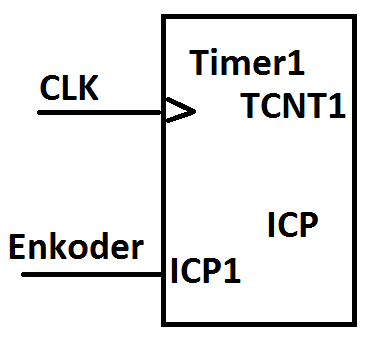
\includegraphics[scale=0.4]{imgs/predkosc.png}
 	\caption[Pomiar częstotliwości obrotu silnika.]{\small{Ilustracja przedstawia ideę pomiaru częstotliwości obrotu silników napędowych. Timer1 jest wewnętrznym, sprzętowym licznikiem mikrokontrolera. Na wyprowadzeniu pinu Atmegi ICP1 podłączony jest enkoder. Licznik taktowany jest wewnętrznym zegarem. W momencie wystąpienia zbocza narastającego na pinie ICP1 aktualna wartość licznika, przechowywana w rejestrze TCNT1, zapisywana jest do rejestru ICR1. Znając szybkość taktowania licznika oraz ilość zliczonych impulsów pomiędzy dwoma narastającymi zboczami enkodera możliwe jest obliczenie częstotliwości obrotu wału silnika.}}
	\label{predkosc}
    \end{center}
  \end{figure}
  Poniższy kod aktywuje opisany wcześniej licznik. Makrodefinicja \_BV() zwraca 8-bitową liczbę z wartością 1 na wskazanej w nawiasie pozycji, np. \_BV(3) = 0000 0100. Pin ICP1 jest 14 pinem mikrokontrolera, najmniej znaczącym bitem rejestru wyjściowego PB. Z racji tego, że może pełnić kilka funkcji należy go odpowiednio zdefiniować. Ustawiany jest jako wejście (poprzez wpisanie do rejestru DDRB (ang. \textit{Data Direction Register B}) wartości 1 na jego pozycji PB0) oraz jest wewnętrznie ściągany do stanu logicznego 0 (poprzez przypisanie wartości 0 w rejestrze PORTB). Znak '\textasciitilde' tworzy bitową negację zapisanej za nią liczby. Operator '\&=' realizuje operację iloczynu bitowego. Kolejnym etapem jest konfiguracja licznika. Służy do tego rejestr TCCR1 (ang. \textit{Timer Counter Control Register 1}) dzielący się na dwie 8-bitowe sekcje: A i B. Ustawienie flagi ICNC1 (ang. \textit{Input Capture Noise Canceler}) rozpoczyna realizację usuwania szumów z odbieranego sygnału. Proces polega na zapamiętywaniu czterech kolejnych próbek sygnału podawanego na pin ICP1. Aktualizacja odczytanego poziomu sygnału przez mikrokontroler odbędzie się dopiero po odebraniu czterech, jednakowych próbek. Ustawienie bitu ICES1 (ang. \textit{Input Capture Edge Select}) nastawia wyzwalanie przechwycenia przy wystąpieniu zbocza narastającego. Timer1 jest licznikiem 16-bitowym. Aby móc prawidłowo odczytać częstotliwość nie można dopuścić aby pomiędzy kolejnymi zboczami sygnału enkodera doszło do przepełnienia licznika (sytuacja ta odpowiada najmniejszej możliwej do odczytania przez układ częstotliwości $f=\frac{f_{clk}}{2^{16}}$).
Dolna granica pomiaru może zostać przesunięta przy wykorzystaniu preskalera, czyli układu realizującego podział częstotliwości. Jego wartość ustawia się w rejestrze TCCR1B poprzez odpowiednią, znajdującą się w nocie katalogowej układu \cite{nota}, konfigurację bitów CS (ang. \textit{Clock Select}). Odbierane z enkodera sygnały mogą pojawić się w dowolnej chwili z dowolną częstością. Niezbędna jest zatem obsługa informacji o ICP1 w przerwaniach. Uruchomienie ich obsługi odbywa się poprzez ustawienie bitu ICIE (ang. \textit{Input Capture Interrupt Enable}) odpowiedzialnego za uruchomienie przerwania związanego z wystąpieniem zdarzenia związanego z wejściem przechwytującym oraz TOIE (ang. \textit{Timer Overflow Interrupt Enable}) związanego z przepełnieniem licznika.
\begin{lstlisting}[caption=Inicjalizacja licznika Timer1 jako układu odmierzącego czas pomiędzy kolejnymi zboczami sygnału podawanego na wejście ICP1]
DDRB &= ~(_BV(PB0));                 ustawienie pinu ICP1 jako wejscie 
PORTB &= ~(_BV(PB0))                 pin przyjmuje wartosc logiczna 0
TCCR1B = _BV(ICNC1) | _BV(ICES1);    ICNC1 - ustawienie filtrowania wejscia ICNC1
                                     ICES1 - wyzwalanie zboczem narastajacym 
TCCR1B |= _BV(CS21) | _BV(CS20);     ustawienie wartosci preskalera na 64
TIMSK1 = _BV(ICIE1) | _BV(TOIE1);    uruchomienie obslugi przerwan
\end{lstlisting}

\namedsection{Generacja sygnału PWM}
Silniki sterowane są przy wykorzystaniu sygnału PWM, który jest generowany sprzętowo przy wykorzystaniu wewnętrznego licznika mikrokontrolera. Czynny udział w tym procesie bierze udział rejestr TCNT0 oraz OCRA0 (ang. \textit{Output Compare Register}, sekcja A). Tak jak w przypadku pomiaru częstotliwości, rejestr TCNT0 przechowuje aktualny stan licznika. Do OCRA0 wpisujemy dowolną, 8-bitową liczbę. W momencie gdy wartość TCNT0 oraz OCRA0 są sobie równe, stan na wyjściu mikrokontrolera (na pinie OC0A) ulega zmianie. W przypadku wpisania do rejestru porównującego wartości 128, otrzymujemy na wyjściu sygnał o wypełnieniu 50~\%. Działanie układu przedstawiono na rysunku \ref{gen_pwn}.
\newpage
\begin{figure}[H]
    \begin{center}
      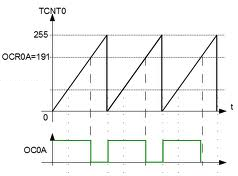
\includegraphics[scale=0.9]{imgs/pwm_gen.png}
 	\caption[Realizacja sygnału PWM.]{\small{Ilustracja przedstawia sposób generowania sygnału PWM przy wykorzystaniu 8-bitowego licznika. W rejestrze TCNT0 znajduje się aktualna wartość licznika, która jest inkrementowana wraz z każdym taktem zegara. Zmienia się od 0 do 255. Do rejestru OCRA0 wpisana jest wartość 191. Jest to wartość porównawcza. W momencie zrównania się wartości OCRA0 oraz TCNT0 sygnał na wyjściu, na pinie OC0A, ulega zmianie.}\footnotemark}
	\label{gen_pwn}
    \end{center}
  \end{figure}  
  	  \footnotetext{\emph{Aplikasi PWM Mikrokontroler ATmega8535}, http://ediamon.files.wordpress.com/,  (data dostępu 03.01.2016 r.)}
\noindent
Poniżej przedstawiono proces inicjalizacji trybu PWM licznika. Kod sprowadza się do odpowiedniego ustawienia bitów rejestrów kontrolnych TCCR. Flagi WGM (ang. \textit{Waveform Generation Mode}) służą do wyboru trybu pracy licznika - zgodnie z dokumentacją techniczną mikrokontrolera\cite{nota}. 
  \begin{lstlisting}[caption=Inicjalizacja generatora PWM przy pomocy licznika Timer2]
TCCR2A |= _BV(WGM20) | _BV(WGM21);   // tryb PWM
TCCR2B =  _BV(CS21) | _BV(CS20);     // preskaler 32
\end{lstlisting}
\noindent
Dodatkowo należy określić częstotliwość generowanego przebiegu, która w tym przypadku wynosi:
\begin{equation}
	f_{PWM} =  \frac{f_{cpu}}{N \cdot 256} = \frac{20 \cdot 10^6}{256 \cdot 32} = 4882 
   \label{eq:czest_kola}
 \end{equation}
 gdzie:  
 \begin{equationDescriptor}
   \EQDitem{$f_{PWM}$}{częstotliwość sygnału PWM [Hz],}
 	\EQDitem{$f_{cpu}$}{częstotliwość taktowania mikrokontrolera [Hz],}
 	 \EQDitem{$N$}{wartość preskalera licznika.}
 \end{equationDescriptor}
\noindent
Dla wyższych częstotliwości tranzystory użyte w mostku H pozostawały w stanie nasycenia - nie realizowały kluczowania. 

Funkcja sterująca generowanym sygnałem pobiera dwa argumenty odpowiedzialne kolejno za obrót w przód oraz w tył. Przez wzgląd na wykonanie mostka H należało wykonać sterowanie przy wykorzystaniu dwóch osobnych sygnałów PWM. Konstrukcja Atmegi pozwala na wytworzenie dwóch przebiegów w oparciu o jeden licznik, przebiegów o tej samej częstotliwości ale innym wypełnieniu. Argumenty pwm\_1 oraz pwm\_2 to wartości porównujące licznika i są przypisywane do rejestrów OCR. Sterują one wypełnieniem sygnału uzyskanego na pinach OC2A (ang. \textit{Output Compare}) i OC2B. Wytworzenie przebiegu jednocześnie na obu pinach zakończyłoby się zwarciem oraz zniszczeniem mostka H. Warunkowa struktura funkcji zabezpiecza układ przed tą możliwością. Dopuszcza generację tylko jednego, określonego sygnału. 
\begin{lstlisting}[caption=Implementacja funkcji sterującej licznikiem Timer2]
void ster_silnik(unsigned char pwm_1, unsigned char pwm_2)
{
	if (pwm_1 == 0x00 && pwm_2 != 0x00 ) //obrot w tyl
	{
		TCCR2A &= ~(_BV(COM2A1)); // zaprzestanie generacji sygnalu
		DDRB &= ~(_BV(PB3)); 	  // ustawienie pinu OCR2A jako wejscie
		PORTB &= ~(_BV(PB3));     // przypisanie wartosci 0
		//ustawienie OCR2B
		TCCR2A |= _BV(COM2B1);    // uruchomienie pinu wyjsciowego
		DDRD |= _BV(PD3);         // ustawienie go jako wyscie
		OCR2B = pwm_2;            // przypisanie wartosci porownujacej
	}
	else if (pwm_2 == 0x00 && pwm_1 != 0x00 ) // obrot w przod
	{
		TCCR2A &= ~(_BV(COM2B1)); // zaprzestanie generacji sygnalu
		DDRD &= ~(_BV(PD3));      // ustawienie pinu OCR2A jako wejscie
		PORTD &= ~(_BV(PD3));     // sciagniecie do GND
		//ustawienie OCR2A
		TCCR2A |= _BV(COM2A1);    // uruchomienie pinu wyjsciowego
		DDRB |= _BV(PB3);         // ustawienie go jako wyjscie
		OCR2A = pwm_1;            // przypisanie wartosci porownujacej
	}
	else // rozlaczenie pinow
	{
		TCCR2A &= ~(_BV(COM2A1) | _BV(COM2A0)); 
		DDRB &= ~(_BV(PB3)); 
		PORTB &= ~(_BV(PB3)); 
		TCCR2A &= ~(_BV(COM2B1) | _BV(COM2B0)); 
		DDRD &= ~(_BV(PD3)); 
		PORTD &= ~(_BV(PD3)); 
	}
}
\end{lstlisting}

\namedsection{Implementacja TWI}
Zastosowane mikrokontrolery posiadają sprzętowe wsparcie dla realizacji komunikacji TWI. Dzięki niej nie ma potrzeby implementowania całej komunikacji od podstaw. Wystarczy jedynie odpowiednia konfiguracja poszczególnych bitów znajdujących się w rejestrze konfiguracyjnym TWCR (ang. \textit{TWI Control Register})\cite{nota}. Flaga: TWEN (ang. \textit{TWI Enable}) ,,uruchamia" TWI, TWIE (ang. \textit{TWI Interrupt Enable}) włącza obsługę przerwania związanego z tym interfejsem, TWEA (ang. \textit{TWI Enable Acknowlage}) steruje generowaniem bitu potwierdzenia. Kolejnym etapem jest przygotowanie 7 bitowego adresu urządzenia. Znajduje się on w rejestrze TWAR (ang. \textit{TWI Address Register}), zapisany na bitach 7..1. Jego wartość, zapisaną w zmiennej ad\_s, należy przesunąć o jedną pozycję w lewo. 
\begin{lstlisting}[caption=Uruchomienie interfejsu TWI oraz przypisanie adresu urządzenia]
TWCR = _BV(TWEN) | _BV(TWIE) | _BV(TWEA);
ad_s = ad_s<<1;  //przesuniecie adresu o jedna pozycje bitowa w lewo
TWAR = ad_s;     //wpisanie przygotowanego adresu
\end{lstlisting}
Układ pracuje w trybie \textit{Slave}, co oznacza, że nigdy nie będzie pierwszy rozpoczynał transmisji a jedynie odpowiadał na zapytania od \textit{Mastera}. Wykrycie przez urządzenie swojego adresu powoduje wyzwolenie przerwania związanego z transmisją TWI. Zmienna TWI\_TWSR zawiera w sobie definicje kodów związanych z poszczególnymi etapami komunikacji. Kody są ściśle określone przez producenta oraz zawarte w nocie katalogowej\cite{nota}. Rejestr TWDR (ang. \textit{TWI Shift Data Register}) przechowuje, odbiera oraz wysyła dane na linię SDA. Poniższy kod służy implementacji trybu nadawczego układu podrzędnego. Kod 0xA8 informuje o tym, że urządzenie nadrzędne chce odczytać z ,,nas" daną (wybrany\_pomiar), którą należy umieścić w rejestrze TWDR. Gotowość urządzenia do transmisji sygnalizujemy ustawieniem flag TWINT, TWEA, TWIE oraz TWEN. Kod 0xB8 służy do wygenerowania bitu potwierdzającego. Natomiast 0xC0 odpowiada za zakończenie transmisji.
\begin{lstlisting}[caption={Fragment przerwania obsługującego komunikację TWI, który jest odpowiedzialny za wysłanie wskazanego bajtu}]
switch(TWI_TWSR)
{
	//slave transmiter
	case TWI_STX_ADR_ACK: //0xA8
		TWDR = wybrany_pomiar(TWI_Buf[0]);
		TWCR = _BV(TWINT) | _BV(TWEA) | _BV(TWIE) | _BV(TWEN);
		break;
	case TWI_STX_DATA_ACK: //0xB8
		TWCR = _BV(TWINT) | _BV(TWIE) | _BV(TWEN);
		break;
	case TWI_STX_DATA_NACK: //0xC0
		TWCR = _BV(TWINT) | _BV(TWEA) | _BV(TWIE) | _BV(TWEN);
		break;
}
\end{lstlisting}
Poniżej znajduje się ciąg dalszy kodu, który jest odpowiedzialny za odbiór informacji. Kod dostosowany jest do przyjmowania dwóch bajtów danych zapisywanych w tablicy TWI\_Buf. Kod 0x60 sygnalizuje poprawną identyfikację adresu podanego na magistralę. Następnie, poprzez ustawienie bitów rejestru TWCR, układ sygnalizuje gotowość do odbioru. Odbiór danych realizowany jest po wystąpieniu kodu 0x80. Zmienna TWI\_INT\_licznik odlicza ilość odebranych danych. Jest ona zerowana przed rozpoczęciem transmisji. Łączność kończy odebranie przez układ sygnału stopu (kod 0xA0). W nim odebrane dane są przypisywane do zmiennych zad\_f\_1 oraz zad\_f\_2, które następnie są przetwarzane w pętli głównej programu.
\begin{lstlisting}[caption={Fragment przerwania obsługującego komunikację TWI, który jest odpowiedzialny za odbiór informacji}]
case TWI_SRX_ADR_ACK: //0x60
	TWI_INT_licznik = 0;
	TWCR = _BV(TWINT) | _BV(TWEA) | _BV(TWIE) | _BV(TWEN);
	break;
	
case TWI_SRX_STOP_RESTART: //0xA0
	TWCR = _BV(TWINT) | _BV(TWIE) | _BV(TWEN) | _BV(TWEA);
	if(TWI_INT_licznik == TWI_wielkosc_ramki)
	{
		zad_f_1 = TWI_Buf[0];
		zad_f_2 = TWI_Buf[1];
	}
	break;

case TWI_SRX_ADR_DATA_ACK: // 0x80
	if(TWI_INT_licznik < TWI_wielkosc_ramki)
		TWI_Buf[TWI_INT_licznik++] = TWDR;
	TWCR = _BV(TWINT) | _BV(TWEA) | _BV(TWIE) | _BV(TWEN);
	break;
\end{lstlisting}

\namedsection{Implementacja regulatora P}
Sterowanie napędem odbywa się przy wykorzystaniu regulatora P, składającego się jedynie z członu proporcjonalnego. Transmitancja, czyli zależność pomiędzy wyjściem a wejściem układu, opisana jest wzorem:
\begin{equation}
	G_{p}(s) =  k_p 
   \label{eq:reg}
 \end{equation}
 gdzie:  
 \begin{equationDescriptor}
   \EQDitem{$G_{p}(s)$}{transmitancja,}
 	\EQDitem{$k_{p}$}{wzmocnienie członu proporcjonalnego.}
 \end{equationDescriptor}
 \noindent
 Na rysunku \ref{schem_ster_2} przedstawiony został schemat blokowy przedstawiający strukturę zaimplementowanego sterownika.
   \begin{figure}[H]
    \begin{center}
      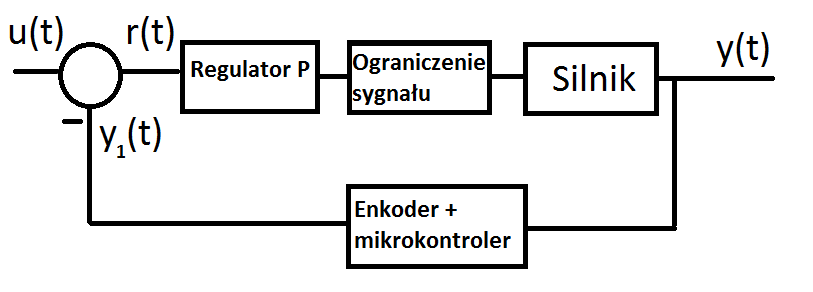
\includegraphics[scale=0.45]{imgs/sterowanie2.png}
 	\caption[Schemat zrealizowanego sterownika.]{\small{Schemat przedstawia układ sterowania silnikami napędowymi. Ujemne sprzężenie zwrotne realizowane jest przy wykorzystaniu enkodera impulsowego, którego sygnał jest interpretowany przez mikrokontroler. Sygnały: $u(t)$ - wartość zadana, $r(t)$ - uchyb, $y(t)$ wyjście układu, $y_1(t)$ - sygnał wyjściowy enkodera.}}
	\label{schem_ster_2}
    \end{center}
  \end{figure}  
Układ charakteryzuje się niezerowym uchybem ustalonym, co w tym przypadku jest do zaakceptowania. Sygnał sterujący regulatora $r(t)$ możemy zapisać jako:
\begin{equation}
	r(t)=u(t)-y_1(t)
   \label{eq:reg1}
 \end{equation}
 gdzie:  
 \begin{equationDescriptor}
   \EQDitem{$r(t)$}{sygnał sterujący regulatorem,}
 	\EQDitem{$u_{t}$}{wartość zadana,}
 	 \EQDitem{$y_1(t)$}{sygnał otrzymany z sprzężenia zwrotnego.}
 \end{equationDescriptor}
 \noindent
Wartość $r(t)$ nazywana jest uchybem, czyli różnicą pomiędzy wartością zadaną a rzeczywistą. Zadaniem regulatora P jest zapewnienie odpowiedniego wzmocnienia tego sygnału. Wartość wypełnienia sygnału PWM zawiera się w przedziale od 0 do 255. Sygnał wyjściowy z regulatora należało odpowiednio ograniczyć. Fragment kodu zaprogramowanego na Atmegach został przedstawiony poniżej. Wzmocnienie regulatora zostało dobrane empirycznie.
\begin{lstlisting}[caption=Program realizujący funkcję regulatora P]
char regulator(char we, char wy)  // we - zadana wartosc, wy - odczytana
{
	int k_p = 30;                 // deklaracja wzmocnienia czlonu P
	int uchyb = 0;                // deklaracja zmiennej uchybu
	int p = 0;                    // deklaracja zmiennej odpowiedzi regulatora
	unsigned char wyjscie = 0;    // deklaracja zmiennej wyjsciowej
	uchyb = (int)(we) - (int)(wy);// obliczanie uchybu
	p = k_p*uchyb;                // obliczanie odpowiedzi regulatora
	if (p > 255)                  // jezeli odpowiedz jest wieksza od 255
	    wyjscie = 0xFF;           // ustaw na wyjsciu wartosc 255
	else if(p < 0)                // jezeli odpowiedz jest mniejsza od 0
	    wyjscie = 0x00;           // ustaw na wyjsciu wartosc 0
	else                          // w przeciwnym wypadku
        wyjscie = (unsigned char)(p);
	return wyjscie;               // zwrocenie wartosci przez funkcje
}
\end{lstlisting}
